%generare il pdf con il comando: pdflatex main.tex
\documentclass[a4paper, oneside, openany, dvipsnames, table]{article}
\usepackage{../template/SWEightStyle}
\usepackage{tabularx}
\newcommand{\mc}{\multicolumn} % handy shortcut macro
\newcolumntype{Z}{>{\centering\arraybackslash}X}
\newcommand{\Titolo}{Manuale Utente}

\newcommand{\Gruppo}{SWEight}

\newcommand{\Approvatore}{Damien Ciagola}
\newcommand{\Redattori}{Alberto Bacco \newline Sebastiano Caccaro \newline Gheorghe Isachi \newline Gionata Legrottaglie}
\newcommand{\Verificatori}{Francesco Corti \newline Francesco Magarotto}

\newcommand{\pathimg}{../template/img/logoSWEight.png}

\newcommand{\Versionedoc}{1.0.0}

\newcommand{\Distribuzione}{\proponente \newline Prof. Vardanega Tullio \newline Prof. Cardin Riccardo \newline Gruppo SWEight}

\newcommand{\Uso}{Esterno}

\newcommand{\NomeProgetto}{Colletta}

\newcommand{\Mail}{SWEightGroup@gmail.com}

\newcommand{\DescrizioneDoc}{Questo documento si occupa di fornire le modalità di utilizzo del software Colletta commissionato}

\usepackage{xcolor}
\usepackage{hyperref}




\begin{document}
\copertina{}
\newpage
\rowcolors{2}{greyROwSWEight}{white}
\section*{Change log}
{
	\renewcommand{\arraystretch}{1.5}
	\centering
	\begin{longtable}{ c c C{6cm} c c }
		\rowcolor{greySWEight}
		\textcolor{white}{\textbf{Version}} & \textcolor{white}{\textbf{Date}} & \textcolor{white}{\textbf{Description}} & \textcolor{white}{\textbf{Author}} & \textcolor{white}{\textbf{Role}}\\
		1.1.1 & 2019-05-08 & Refactor §\ref{sec:BackArchi}  & Francesco Corti & \reda{}\\
		1.1.0 & 2019-05-06 & Refactor §\ref{sec:FrontArchi} & Sebastiano Caccaro & \reda{}\\
		1.0.1 & 2019-05-06 & Fixed §\ref{fig:UMLFront} & Sebastiano Caccaro & \reda{}\\
		1.0.0 & 2019-04-10 & Document approval and release & Damien Ciagola & \RdP{}\\
		0.4.0 & 2019-04-04 & Checking & Gheorghe Isachi & \ver{}\\
		0.4.0 & 2019-04-02 & §1 completed  & Francesco Corti & \reda{}\\		
		0.3.0 & 2019-04-02 & §2 and §3 completed  & Francesco Magarotto & \reda{}\\				
		0.2.0 & 2019-04-01 & §4 completed  & Sebastiano Caccaro & \reda{}\\
		0.1.1 & 2019-04-01 & Written §4 to §4.2.1  & Sebastiano Caccaro & \reda{}\\
		0.1.0 & 2019-04-01 & Backbone translated in English & Sebastiano Caccaro & \reda{}\\
		0.0.1 & 2019-03-18 & Document backbone & Enrico Muraro & \reda{}\\
		
	\end{longtable}

}


\newpage
\tableofcontents
\newpage
\listoffigures

\newpage
\subsection{Document goal}
The purpose of this document is to provide all the necessary information to extend, correct and improve Colletta.
There will be additional information regarding setting up the development environment to work in an environment that is as consistent as possible with that used
by the other members of group SWEight, but can be ignored if you only want to use part of the product.
This guide was written taking into account the Microsoft Windows and Linux operating systems. If other systems are used, compatibility issues may arise, even if it's unlikely. In this case refer to the git page. This document will grow as the product will be fully
developed.

\subsection{Product goal}
The purpose of the product is the creation of a collaborative data collection platform where users can prepare and/or perform small grammar exercises. 
The front-end of the system consists of a web application developed with React and Redux, while the back-end is a Spring Boot application written in Java, which will handle HTTP Requests sent from the front-end. 

\subsection{References}


\subsubsection{Installation references}

\begin{itemize}
\item \textbf{Git}: \url{https://git-scm.com/}
\item \textbf{Node.js}: \url{https://nodejs.org/en/}
\item \textbf{NPM}: \url{https://www.npmjs.com/}
\item \textbf{Oracle JDK}: \url{https://www.oracle.com/technetwork/java/javase/downloads/index.html}
\item \textbf{OpenJDK}: \url{https://openjdk.java.net/}
\item \textbf{Maven}: \url{https://maven.apache.org/}
\item \textbf{Lombok}: \url{https://projectlombok.org/}
\item \textbf{VSCode}: \url{https://code.visualstudio.com/} 

\end{itemize}

\subsubsection{Legal references}
\begin{itemize}
\item \textbf{MIT License}: \url{https://opensource.org/licenses/MIT}
\end{itemize}

%\subsubsection{Informative references}


\newpage
\section{Requisiti}

    Di seguito vengo riportati i requisiti minimi per garantire il funzionamento del prodotto: 
\textbf{Colletta: piattaforma raccolta dati di analisi di testo}. 


\subsection{Requisiti software}
\begin{itemize}
\item \textbf{Sistema operativo}: qualsiasi;
\item \textbf{Browser web}: ogni browser web aggiornato all'ultima versione. Per garantire il funzionamento della piattaforma vengono elencate le versioni minime compatibili:
	\begin{itemize}
		\item \textbf{Chrome}: 60;
		\item \textbf{Edge}: 13;
		\item \textbf{Firefox}: 55;
		\item \textbf{Opera}: 47;
		\item \textbf{Safari}: 11.1.
	\end{itemize}
\end{itemize}
Per i browser sotto queste versioni non si garantisce l'accesso alla piattaforma. Si specifica inoltre che \texttt{JavaScript} deve essere abilitato nel browser per il corretto funzionamento dell'applicazione.

\subsection{Requisiti hardware}
L'unico requisito hardware necessario per il corretto funzionamento dell'applicazione è che sia presente una connessione ad Internet. 
\newpage


\newpage
\section{Istruzione per l'utilizzo}
  L'header della {dashboard}\ped{G} è uguale come struttura per ogni tipo di utente. Su di esso troviamo un link che porta alla modifica dei dati personali, chiamato \textit{Profilo}, e un link, \textit{Esci}, che, se cliccato, effettua il logout dal sistema.



\subsection{Interfaccia}
    \begin{figure}[H]
        \centering
   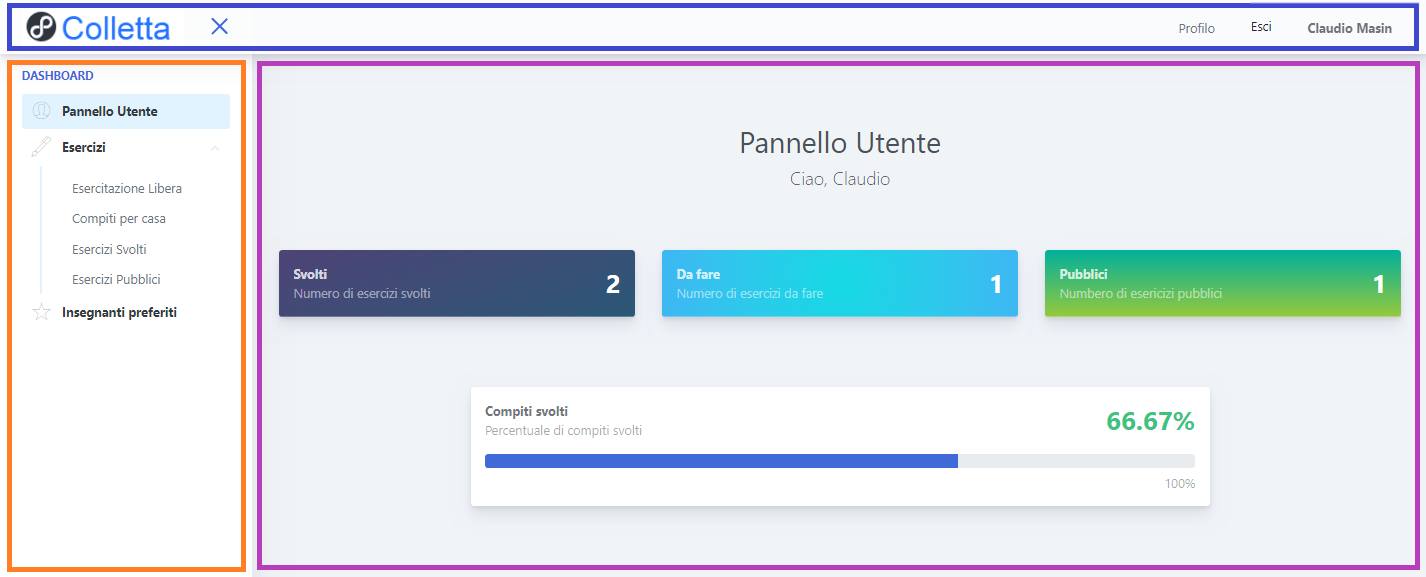
\includegraphics[width=17cm]{sez/img/istruzioni/panoramica.png} 
        \caption{Panoramica dell'interfaccia}\label{fig:1}
    \end{figure}
  La struttura generale di una pagina è la stessa per ogni utente loggato. Sono presenti i seguenti elementi di base:
    \begin{itemize}
        \item Barra del menu;
        \item {Sidebar}\ped{G};
        \item Contenuto della pagina.
    \end{itemize}
 A seconda del tipo di utente (Allievo, Insegnante, Sviluppatore, Amministratore) e della pagina selezionata, verranno visualizzati a schermo contenuti diversi. Ogni utente ha comunque a disposizione lo stesso header e un link al suo pannello utente.


\subsection{Utente non autenticato}
    \subsubsection{Registrazione}
    	\begin{figure}[H]
        	\centering
        	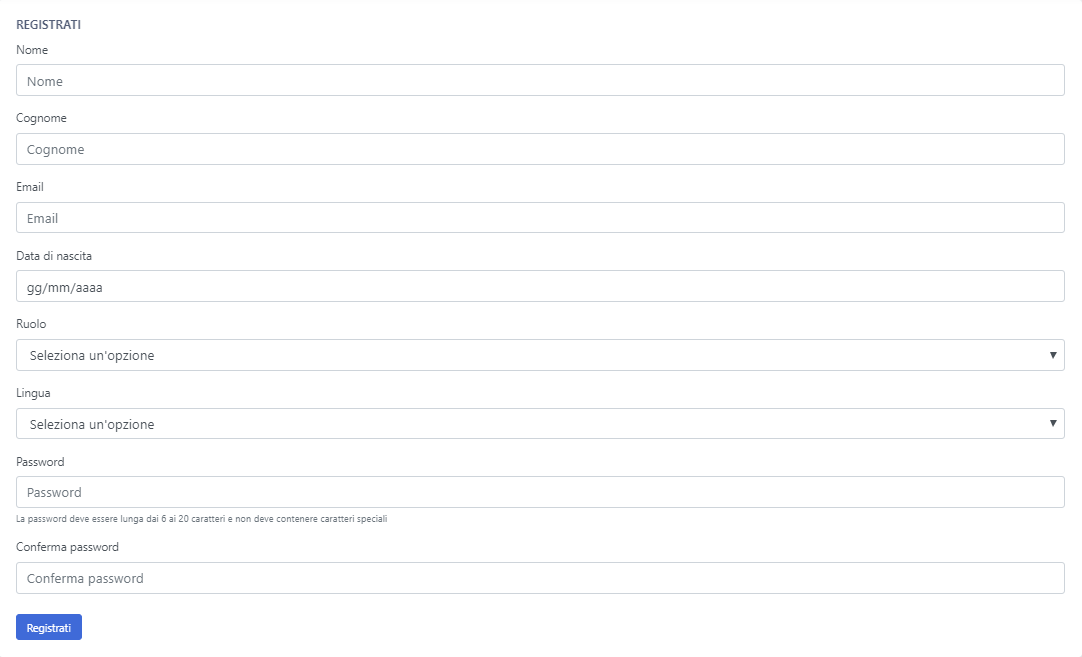
\includegraphics[width=1\linewidth]{sez/img/autenticazione/formRegistrazione.PNG} 
        	\caption{Form per la registrazione}\label{fig:registrazione}
    	\end{figure}
	  Se non si è ancora registrati è possibile farlo cliccando sul bottone \textit{Registrati} presente nella barra del menu. Una volta compilato il form viene inviata una mail per l'attivazione dell'account. E' necessario cliccare sul link appena ricevuto, successivamente verrà aperta una pagina con un messaggio di conferma. A questo punto se il ruolo scelto è \textit{Insegnante} o \textit{Allievo} è possibile accedere alla piattaforma; se \textit{Sviluppatore} è necessario attendere anche l'attivazione manuale da parte di un  \textit{Amministratore} della piattaforma. I dati sono tutti obbligatori e il form visualizzato è quello in \autoref{fig:registrazione}.\\
    \subsubsection{Login}
    	\begin{figure}[H]
        	\centering
        	
\includegraphics[width=1\linewidth]{sez/img/autenticazione/formAccedi.PNG} 
        	\caption{Dati per effettuare l'accesso}\label{fig:1}
    	\end{figure}
 	  Dopo aver effettuato la registrazione si accede cliccando su \textit{Accedi} nella barra del menu. E' necessario inserire email e password e successivamente cliccare sul pulsante \textit{Accedi} del form.


% UTENTE AUTENTICATO
\subsection{Utente autenticato generico}

    \subsubsection{Logout}
    Per effettuare il {logout}\ped{G} si deve cliccare sulla voce \textit{Esci} dalla barra del menu. Facendo ciò, l'utente termina la propria sessione.
    \subsubsection{Modifica dati}
    Cliccando su \textit{profilo} l'utente ha la possibilità visualizzare e modificare i propri dati tramite un form simile a quello di registrazione. L'utente non può modificare il proprio ruolo dopo l'iscrizione.

    \subsection{Allievo}
      L'allievo si iscrive nel portale Colletta per svolgere esercizi di analisi grammaticale. Può svolgere esercizi assegnati da un'insegnante o svolgere esercizi utilizzando la correzione automatica del sistema. L'allievo ha poi la possibilità di confrontare la sua soluzione con quella presentata dal sistema.
        \subsubsection{Sidebar}
          La sidebar dell'allievo presenta le seguenti voci:
            \begin{itemize}
                \item Pannello utente;
                \item Esercitazione libera;
                \item Compiti per casa;
                \item Esercizi svolti;
                \item Esercizi pubblici;
                \item Insegnanti preferiti.
            \end{itemize}
            

            
        \subsubsection{Pannello utente}
          Il pannello utente è un riassunto di tutti i progressi e le attività svolte dall'allievo. Al momento il pannello utente mostra un messaggio di benvenuto, l'allievo è quindi libero di selezionare una delle voci di menu ed esercitarsi.
        	\begin{itemize}
        		\item Esercizi svolti;
        		\item Esercizi da svolgere;
        		\item Esercizi pubblici disponibili;
        	\end{itemize}
        
          \begin{figure}[H]
        	\centering
        	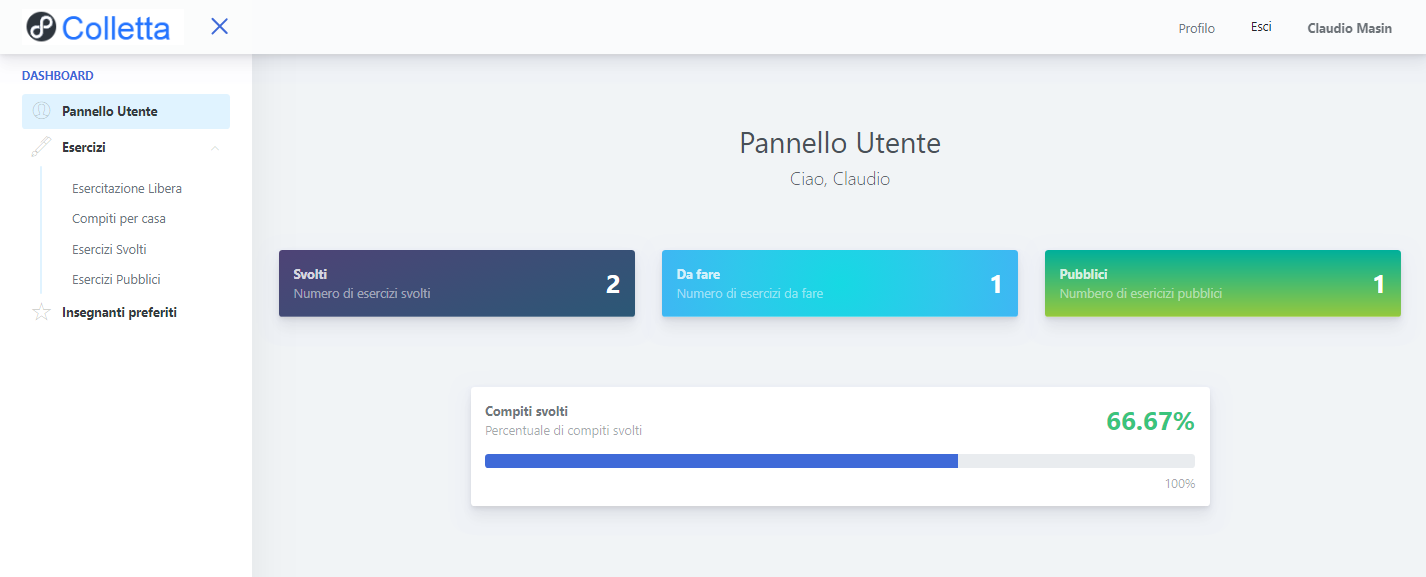
\includegraphics[width=1\linewidth]{sez/img/studente/pannello.png} 
        	\caption{Pannello utente - Studente}\label{fig:1}
    	  \end{figure}
               
	\newpage
        \subsubsection{Esercitazione libera}      
        	\begin{figure}[H]
                \centering
                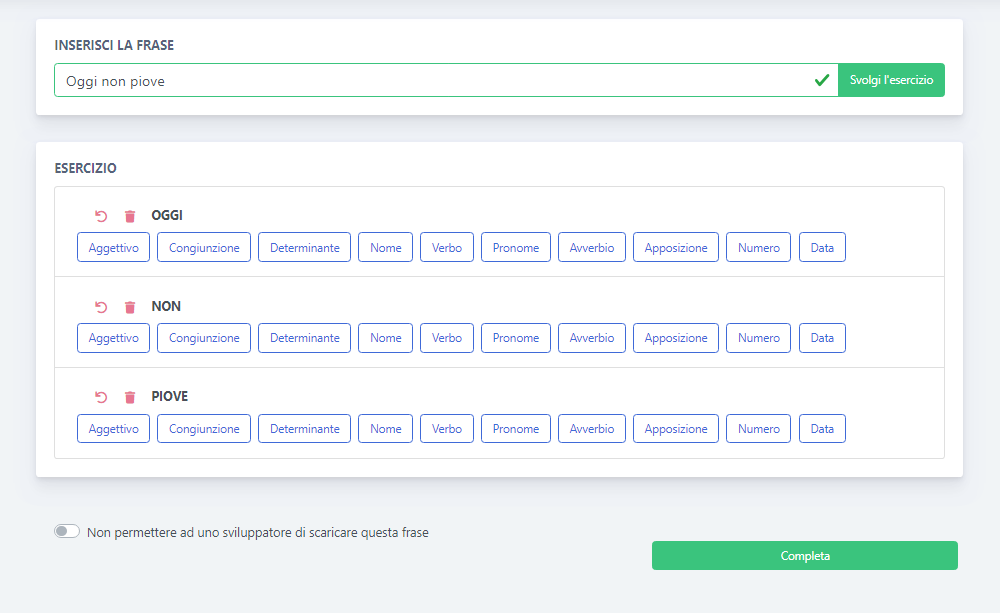
\includegraphics[width=17cm]{sez/img/studente/esercitazioneLiberaEsegui.PNG} 
                \caption{Svolgimento esercizio libero}\label{fig:1}
        	\end{figure}
          In questa pagina è possibile svolgere un esercizio inserendo nella casella di testo una frase da analizzare. La soluzione appena inserita viene confrontata con quella generata automaticamente.
        \\ Svolgimento:
        	\begin{enumerate}        
            	\item Scrivere la frase da analizzare all'interno della casella di testo;
            	\item Cliccare su \textit{Svolgi l'esercizio};
            	\item Svolgere l'esercizio e cliccare \textit{Completa}.
        	\end{enumerate}
        	\label{sec:esLib}
        	Lo svolgimento dell'esercizio è guidato;ogni pulsante rappresenta una scelta possibile, il primo pulsante selezionato corrisponde alla categorica alla quale appartiene la parola, le scelte successive raffinano l'analisi. Ad ogni click di un pulsante vengono generati dei pulsanti strettamente collegati a quello precedente. In caso non comparissero più pulsanti, significa che l'analisi per quella parola è terminata. In ogni momento l'allievo può decidere di resettare la soluzione per una determinata parola (icona cestino), o annullare l'ultima scelta (freccia indietro).        \linebreak	
        A sinistra del pulsante completa è presente un flag che indica se la frase appena inserita può essere messa a disposizione degli sviluppatori che utilizzano i dati della piattaforma; non selezionandolo si acconsente la condivisione di questo dato.
        	

      
        \newpage
  		\subsubsection{Compiti per casa}
 		  In questa sezione l'allievo ha la possibilità di visualizzare gli esercizi a lui assegnati e sceglierne uno da svolgere.
        	\begin{figure}[H]
            	\centering
            	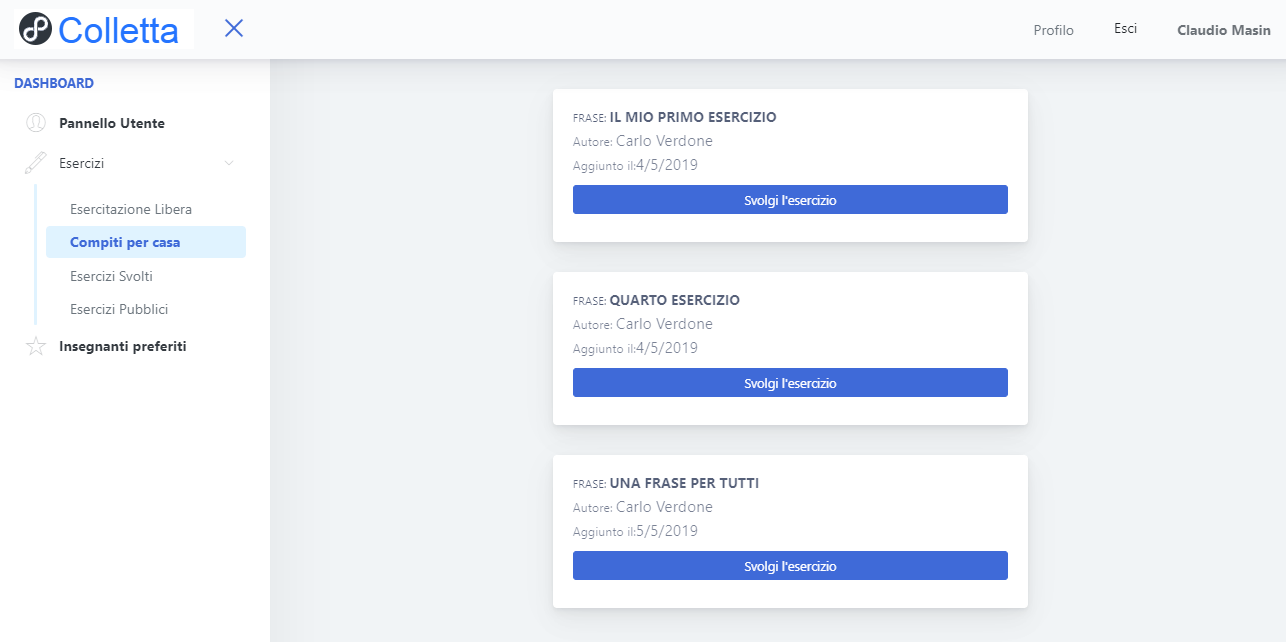
\includegraphics[width=17cm]{sez/img/studente/compitopercasa.PNG} 
            	\caption{Scelta esercizio da svolgere}\label{fig:1}
        	\end{figure}

		  E' possibile scegliere l'esercizio da svolgere cliccando sul pulsante \textit{Svolgi l'esercizio}. Una volta selezionato l'esercizio di apre una pagina per lo svolgimento, contenente un set di scelte per ogni parola appartenente alla frase dell'esercizio.     
       
        	\begin{figure}[H]
            	\centering
            	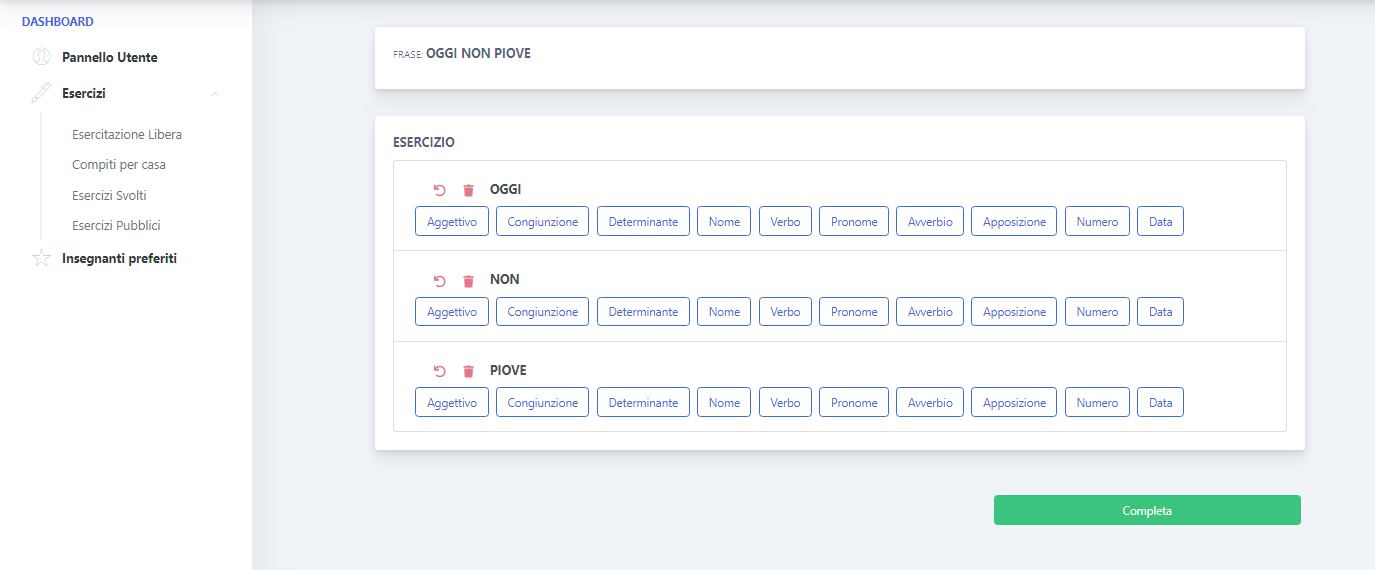
\includegraphics[width=17cm]{sez/img/studente/svolgimentoesercizio.PNG} 
            	\caption{Svolgimento esercizio}\label{fig:1}
        	\end{figure}      
	L'allievo esegue quindi l'analisi della frase allo stesso modo descritto in \S\ref{sec:esLib}. La soluzione visualizzata alla fine sarà in questo caso quella dell'insegnante che ha assegnato l'esercizio. \newpage
	
	Le scelte uguali a quelle della soluzione dell'insegnante vengono evidenziate in verde mentre quelle diverse in rosso. In alto a destra viene mostrato il voto in decimi calcolato automaticamente paragonando la soluzione con quella dell'insegnante.
	
	\begin{figure}[H]
            	\centering
            	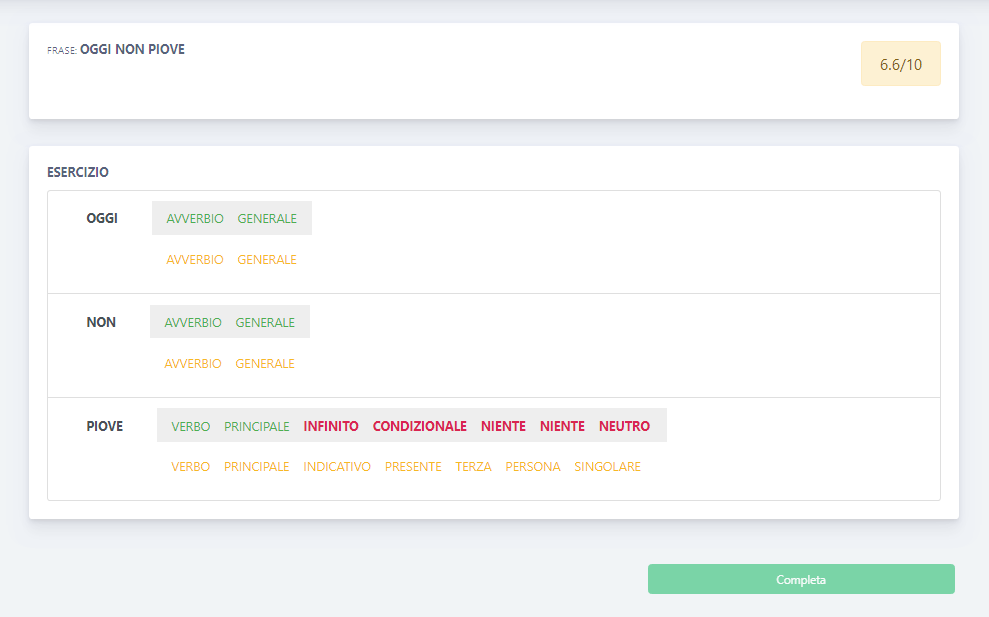
\includegraphics[width=17cm]{sez/img/studente/risultatoEsercizio.png} 
            	\caption{Risultato esercizio svolto}\label{fig:1}
        	\end{figure}
        
        
        
        \subsubsection{Esercizi svolti}
                 In questa pagina è possibile visualizzare lo storico degli esercizi che sono stati svolti. Per ogni esercizio svolto sono visualizzabili la data di aggiunta, la frase analizzata e il nome dell'insegnante che ha assegnato l'esercizio.
        	\begin{figure}[H]
            	\centering
            	
\includegraphics[width=17cm]{sez/img/studente/esercizisvolti.PNG} 
            	\caption{Storico esercizi svolti}\label{fig:1}
        	\end{figure}
 
        
\newpage
    \subsection{Insegnante}
      L'insegnante è l'utente che può inserire esercizi privati o decidere di assegnarli ai propri allievi. 
        \subsubsection{Sidebar}
          La sidebar dell'insegnante presenta le seguenti voci:
        	\begin{itemize}
            	\item Pannello utente;
            	\item Inserisci esercizio;
            	\item Esercizi inseriti;
            	\item Esercizi allievi.
        	\end{itemize}
        
        
        
        \subsubsection{Pannello utente}
          Il pannello utente mostra un messaggio di benvenuto all'insegnante, un riepilogo con il numero di esercizi inseriti, le classi create e gli studenti presenti nel sistema.
        
        \begin{figure}[H]
            	\centering
        		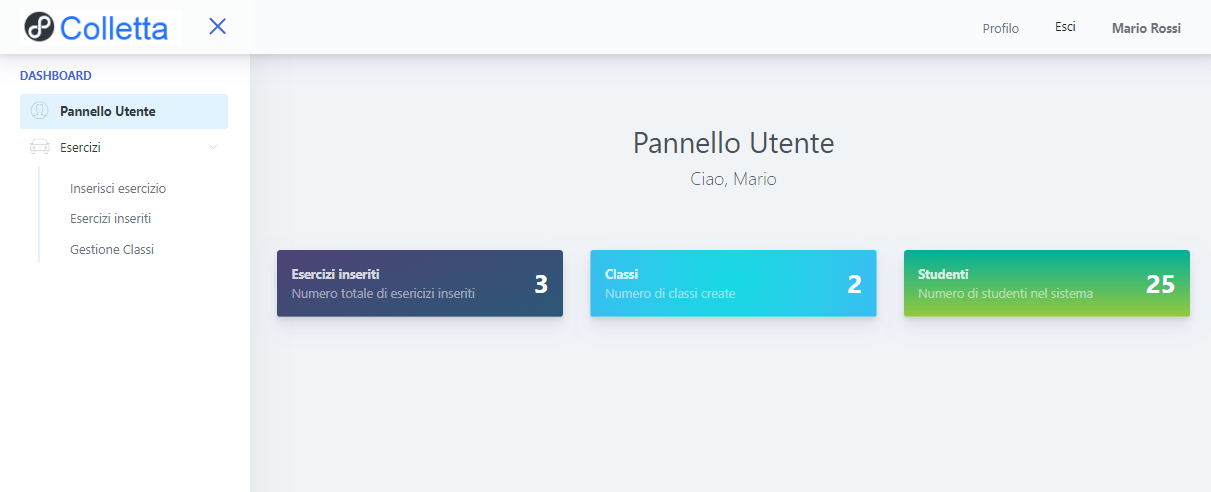
\includegraphics[width=17cm]{sez/img/insegnante/pannello.png} 
            	\caption{Pannello utente - Insegnante}\label{fig:1}
        	\end{figure}
        	
        \subsubsection{Inserisci esercizio}
          Il compito principale dell'insegnante è quello di inserire esercizi all'interno del sistema ed assegnarli agli alunni.
        	\begin{figure}[H]
            	\centering
        		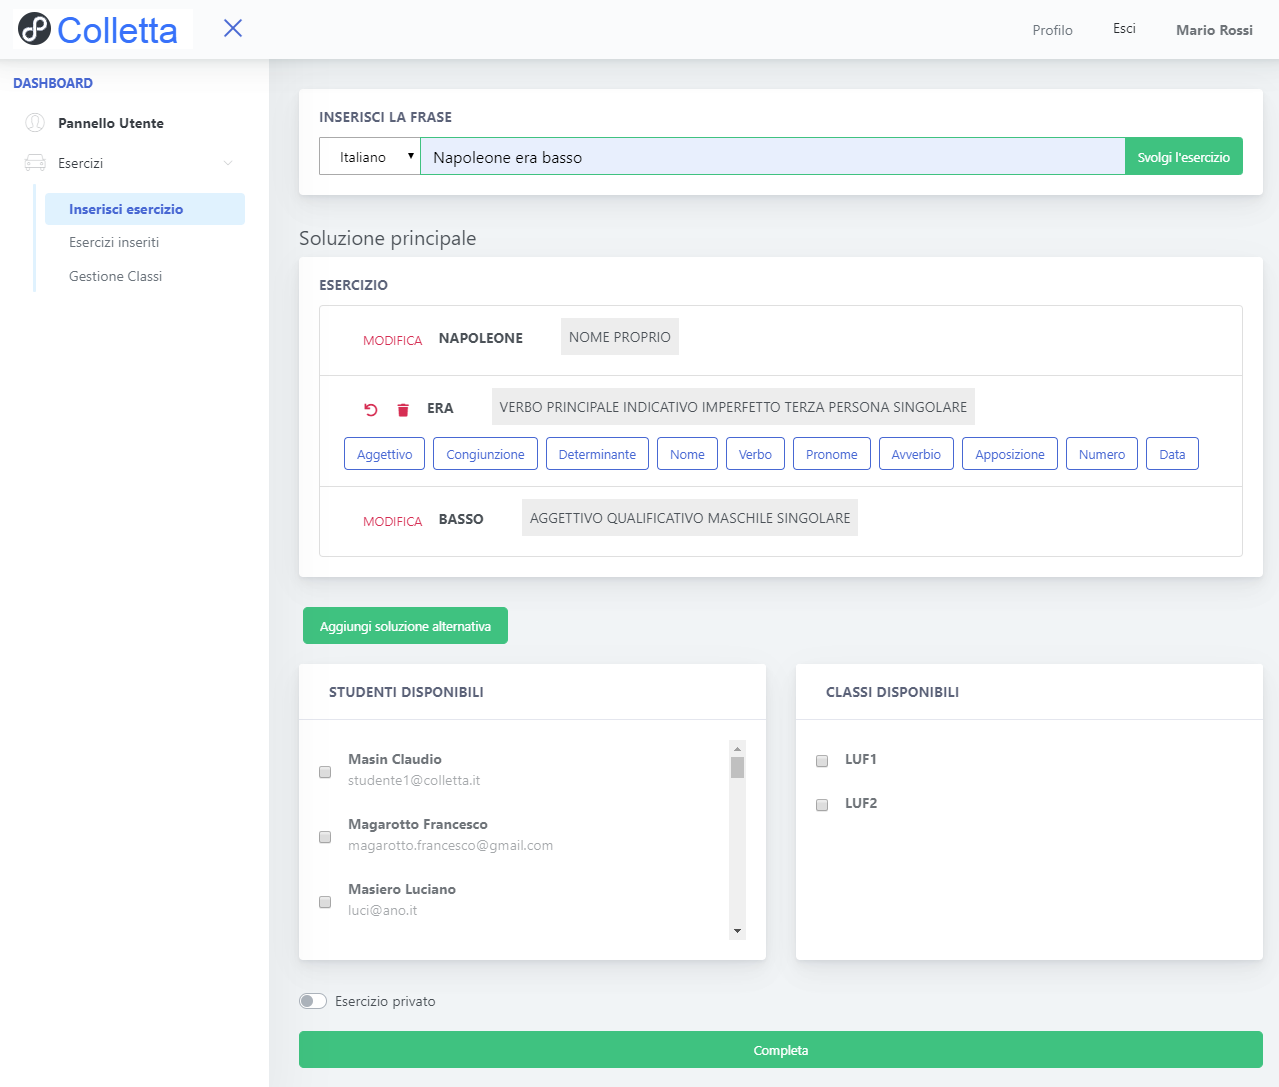
\includegraphics[width=17cm]{sez/img/insegnante/inserisciEsercizio.PNG} 
            	\caption{Inserimento e assegnazione esercizio}\label{fig:1}
        	\end{figure}
        
          Dopo aver inserito la frase, verrà visualizzata la correzione automatica. Se è ritenuto necessario è possibile modificare la soluzione cliccando sul pulsante \textit{Modifica}; se cliccato, viene eliminata la soluzione proposta dal sistema per quella parola e chiesto di inserire una nuova soluzione. Durante l'inserimento manuale della soluzione l'insegnante ha la possibilità di tornare indietro di un passo o di resettare completamente la soluzione appena inserita. Questo processo è analogo a quello presentato in \S\ref{sec:esLib}. 
          Se è necessario, è possibile inserire una soluzione alternativa; cliccando sul pulsante \textit{Aggiungi soluzione alternativa} si apre un box identico a quello della soluzione principale; la modalità dell'inserimento della soluzione infatti è la stessa della soluzione principale.  \linebreak \linebreak Finita la correzione, l'insegnate può assegnare l'esercizio a un allievo selezionandolo dalla lista a sinistra sotto le soluzioni inserite oppure può assegnarlo direttamente ad una classe di studenti precedentemente creata selezionandola dall'elenco a destra sotto le soluzioni. \linebreak \linebreak
          Prima di completare l'inserimento dell'esercizio, si può scegliere se aggiungere l'esercizio nella lista degli esercizi pubblici, disponibili agli alunni a cui non è stato assegnato e se dare la possibilità agli sviluppatori che utilizzano i dati raccolti dalla piattaforma di scaricare anche quest'ultimo. \linebr  Cliccando sul pulsante \textit{Completa} l'esercizio viene aggiunto al sistema.
          
        
        
        
        \subsubsection{Esercizi inseriti}
        
        Funzionalità al momento non disponibile. Questa sezione permette di visualizzare tutti gli esercizi inseriti, si possono vedere la frase inserita e la data di aggiunta.
        
        
        
        
        \subsubsection{Esercizi allievi}        
         Funzionalità al momento non disponibile. In questa sezione sono visibili i risultati dagli allievi.
        
        
        
        
	\newpage
    \subsection{Sviluppatore}
    Lo sviluppatore si iscrive al sito perché interessato a scaricare i dati prodotti dagli utenti durante l'esecuzione di esercizi di analisi grammaticale.
    	\subsubsection{Sidebar} 
    	  La sidebar dello sviluppatore presenta le seguenti voci:
    		\begin{itemize}
    			\item Pannello utente;
    			\item Pannello sviluppatore.
    		\end{itemize}
    
    
    
    
    	\subsubsection{Pannello utente}
    	  Il pannello utente mostra un messaggio di benvenuto allo sviluppatore, che è libero di procedere allo scaricamento dei dati prodotti dagli utenti.



    	\subsubsection{Pannello sviluppatore}
    		\begin{figure}[H]
				\centering
				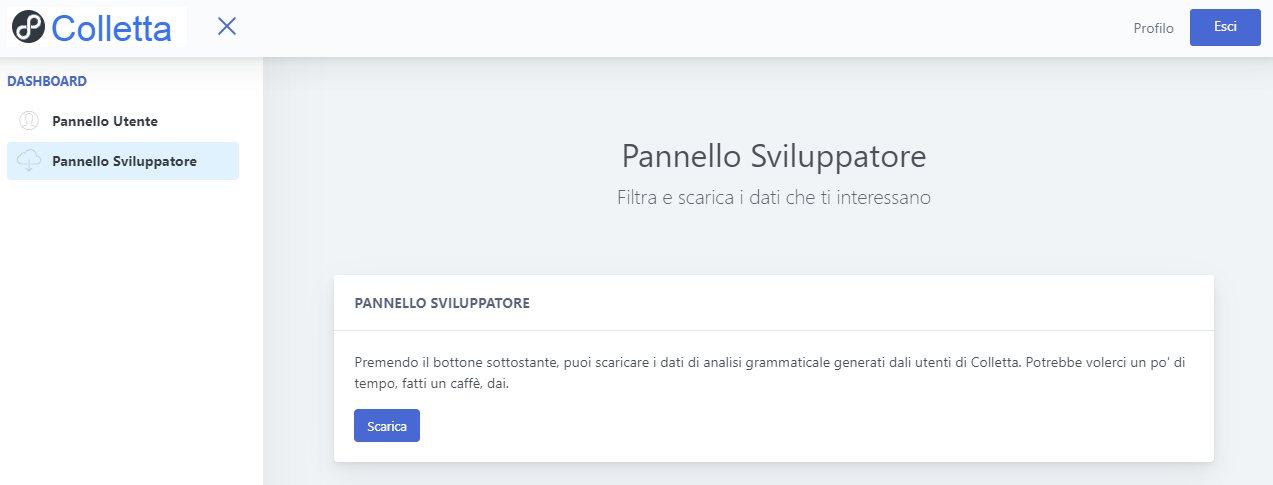
\includegraphics[width=17cm]{sez/img/sviluppatore/datipronti.png}
				\caption{Scaricamento dati disponibili}\label{fig:1}
			\end{figure}
		  Cliccando sul bottone di \textit{Scarica}, lo sviluppatore può scaricare i dati prodotti dagli utenti, avrà successivamente la possibilità di filtrare questi dati.




	\newpage
	\subsection{Amministratore}
	L'amministratore ha la possibilità di gestire tutti gli utenti che non siano amministratori; inoltre può approvare o declinare le richieste di iscrizione degli sviluppatori.
		\subsubsection{Sidebar}
		  Voci nella sidebar:
			\begin{itemize}
				\item Pannello utente;
				\item Sviluppatori;
				\item Utenti.
			\end{itemize}



		\subsubsection{Pannello utente}
		 Il pannello dà il benvenuto allo sviluppatore, che è libero di procedere alla gestione degli utenti.




		\subsubsection{Sviluppatori}
			\begin{figure}[H]
				\centering
				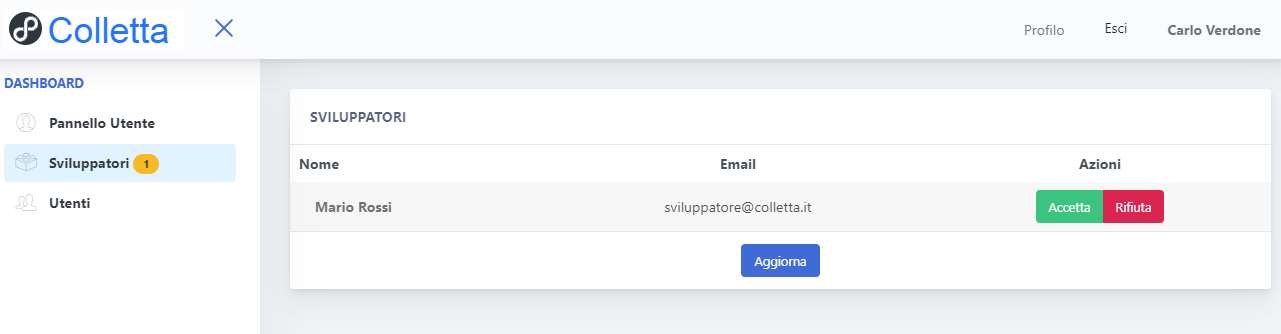
\includegraphics[width=17cm]{sez/img/amministratore/conf_ric_svil.PNG}
				\caption{Richieste di iscrizione degli sviluppatori}\label{fig:1}
			\end{figure}
		  In questa pagina l'amministratore può approvare o rifiutare le richieste di iscrizione degli sviluppatori. Viene presentata una lista contente gli sviluppatori che hanno richiesto di iscriversi al sistema. Ogni sviluppatore ha un nome e una mail. L'amministratore, premendo su \textit{Accetta}, consente allo sviluppatore di fare il login; se invece preme su \textit{Rifiuta}, l'amministratore cancella lo sviluppatore dal sistema. Premendo su \textit{Aggiorna}, l'amministratore aggiorna la lista di sviluppatori.


		\subsubsection{Utenti}
			\begin{figure}[H]
				\centering
				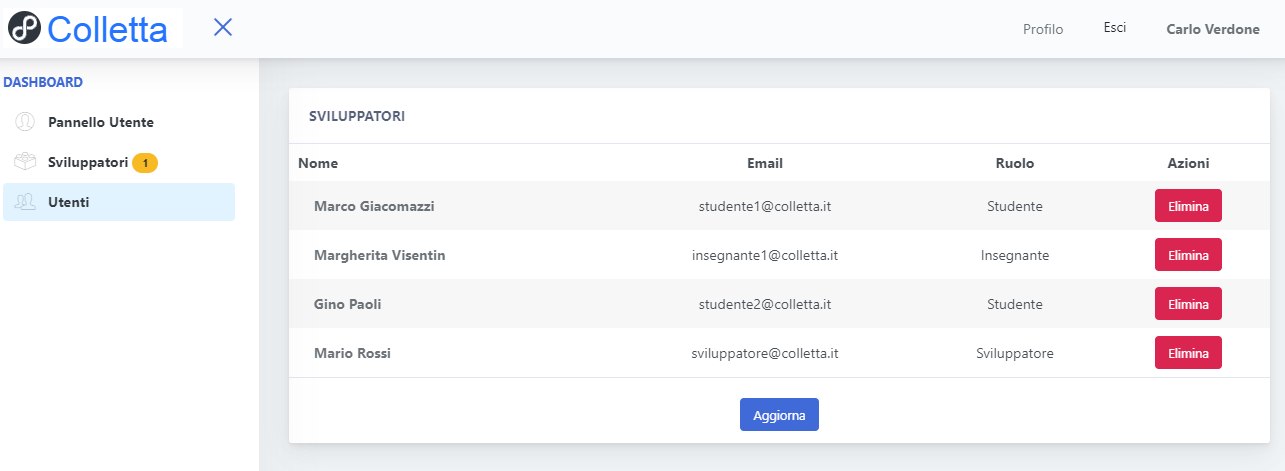
\includegraphics[width=17cm]{sez/img/amministratore/gestisciutenti.PNG}
				\caption{Gestione utenti}\label{fig:1}
			\end{figure}
		  In questa pagina l'amministratore può visualizzare gli utenti iscritti ed eventualmente eliminarli dal sito. Per ogni utente sono presenti nome, email e ruolo (Insegnante, Sviluppatore o Allievi). Gli amministratori non figurano in questo elenco. L'amministratore, cliccando su \textit{Elimina}, può cancellare un utente dal sistema. Premendo su \textit{Aggiorna}, l'amministratore aggiorna la lista di utenti.


\appendix
\addcontentsline{toc}{part}{Appendici}
\newpage
\section{Glossario}
\textbf{Dashboard:}\\La schermata di gestione e monitoraggio dei dati a disposizione.

\textbf{Logout:}\\Plusante per uscire dal sito, ritornando alla pagina di Login. 

\textbf{Sidebar:}\\ La sezione a sinistra della pagina con il menu delle azioni che sono messe a disposizione all'utente.
\end{document}
